\chapter{Recognition of Bricks}


\begin{figure}[H]
    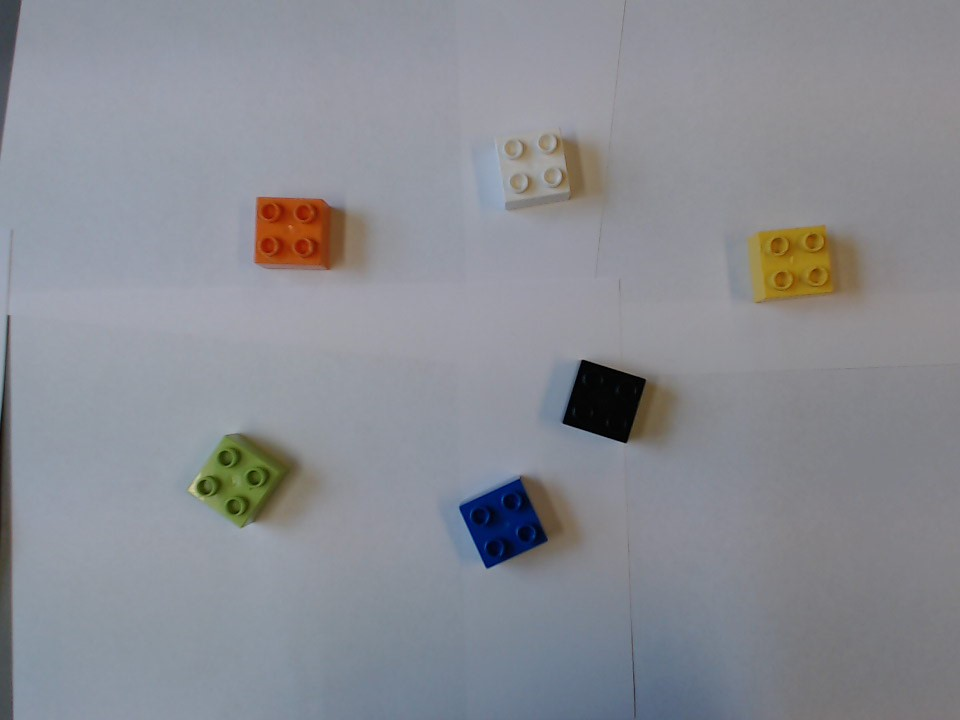
\includegraphics[width=0.4\textwidth]{figures/RealLego4.jpg}
    \caption{}
    \label{fig:RealLego4}
\end{figure}

Convert the image to HSV and split the channels.

To find the color blocks (orange, yellow, green and blue) the saturation channel is used combined with a threshold to find the pixels that have a high saturation value (bright colors). This step results in a binary mask.

\begin{figure}[H]
    \captionbox  %<--use captionbox instead if no global caption is needed
    {               %                                \%-%-%-%-%-%-%\               
        \label{fig:saturation}                                  
    }                                                                 
    {                                                                  
        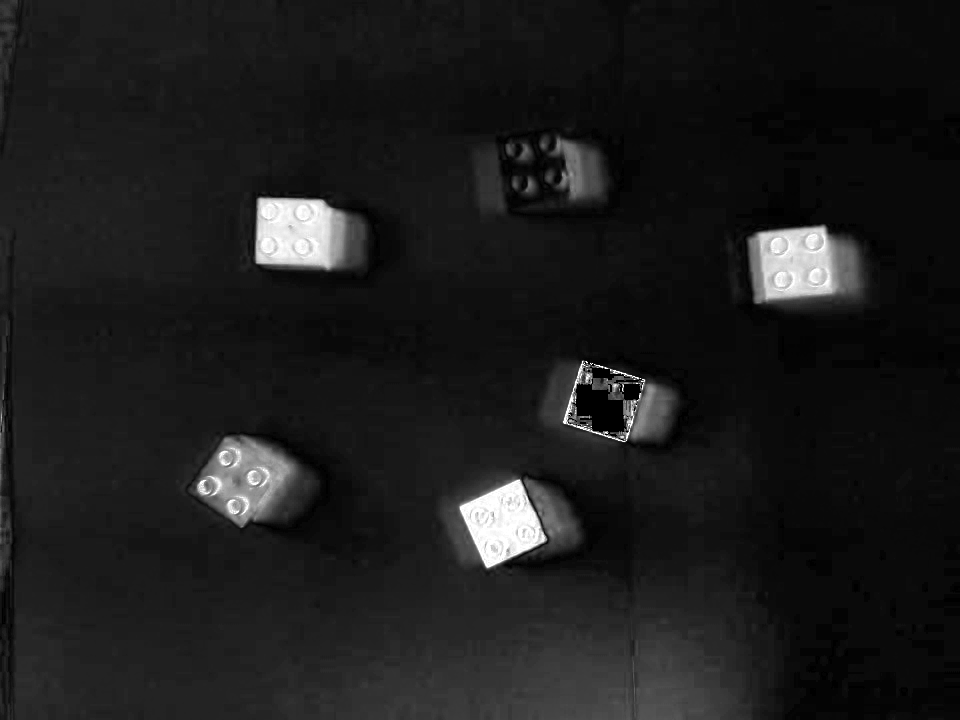
\includegraphics[width=.4\textwidth]{figures/saturation.png}         
    }                                                                    
    \hspace{5pt}                                                          
    \captionbox
    {       
        \label{fig:colour_mask}                                     
    }
    {
        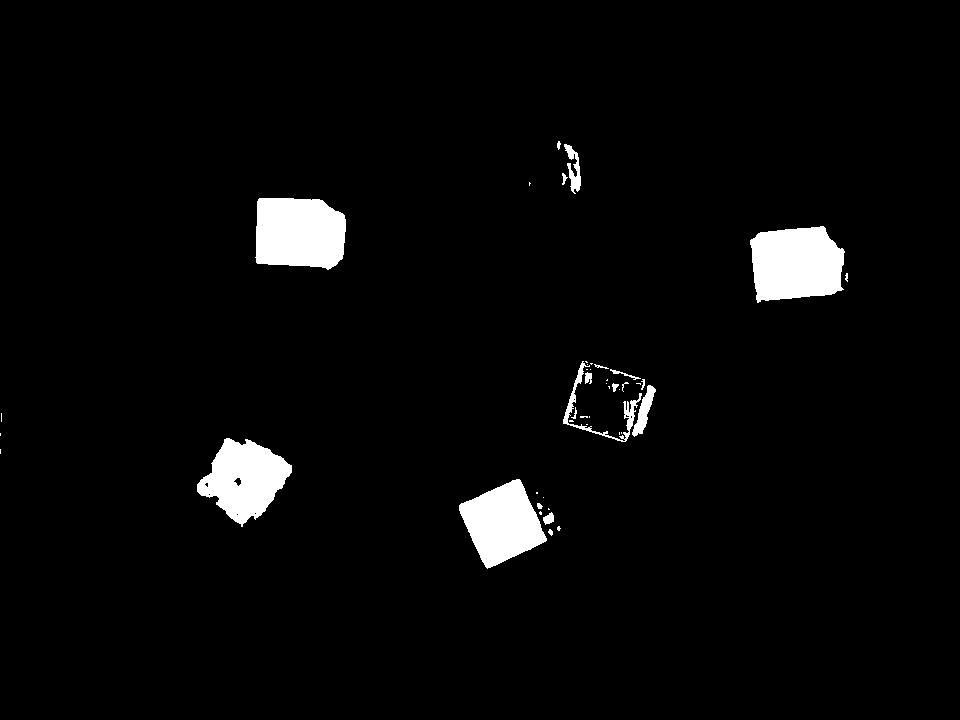
\includegraphics[width=.4\textwidth]{colour_mask.png}            
    }                                                                             
\end{figure}

To fin the black bricks for Homer, the value channel can be used to find the pixels with very low value.

\begin{figure}[H]
    \captionbox  %<--use captionbox instead if no global caption is needed
    {               %                                \%-%-%-%-%-%-%\               
        \label{fig:value}                                  
    }                                                                 
    {                                                                  
        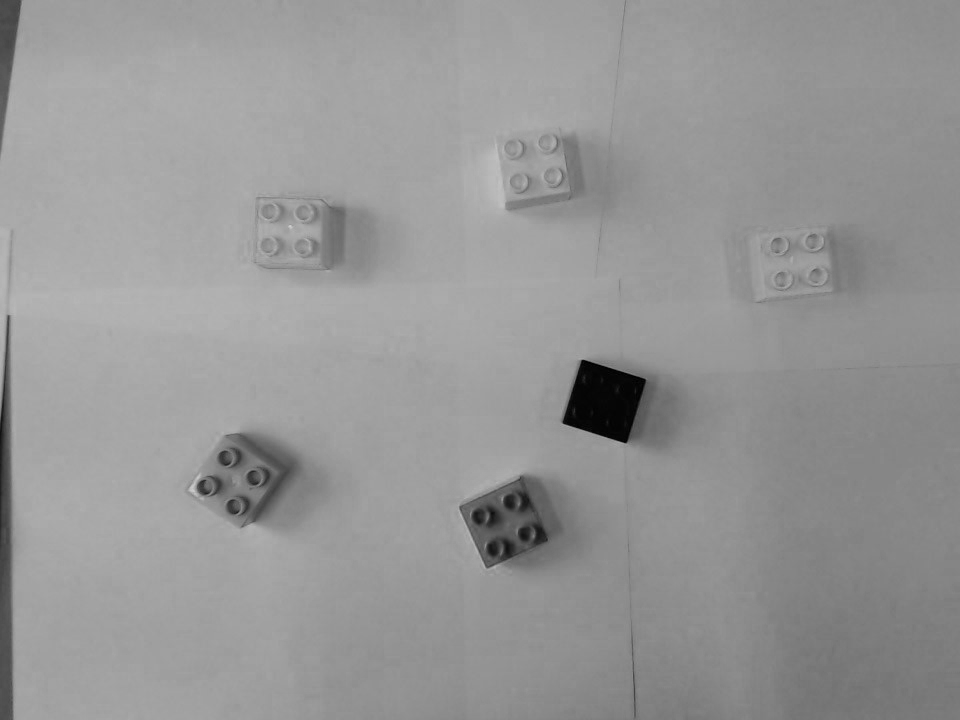
\includegraphics[width=.4\textwidth]{figures/value.png}         
    }                                                                    
    \hspace{5pt}                                                          
    \captionbox
    {       
        \label{fig:black_mask}                                     
    }
    {
        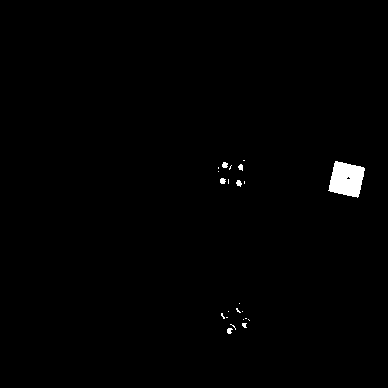
\includegraphics[width=.4\textwidth]{black_mask.png}            
    }                                                                             
\end{figure}

Combining the two masks, the final one can be found as seen in \autoref{fig:final_mask}. To enhance the mask, an opening operation to remove some of the noise, followed by a closing operation to fill possible holes in the objects. This operations give the result presented on \autoref{fig:final_mask2}.

\begin{figure}[H]
    \captionbox  %<--use captionbox instead if no global caption is needed
    {               %                                \%-%-%-%-%-%-%\               
        \label{fig:final_mask}                                  
    }                                                                 
    {                                                                  
        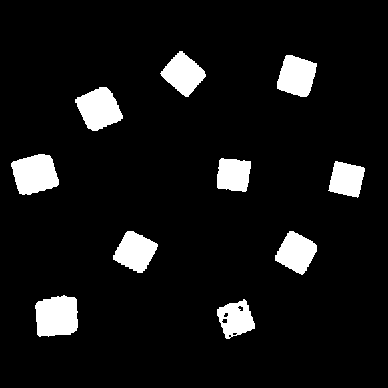
\includegraphics[width=.4\textwidth]{figures/final_mask.png}         
    }                                                                    
    \hspace{5pt}                                                          
    \captionbox
    {       
        \label{fig:final_mask2}                                     
    }
    {
        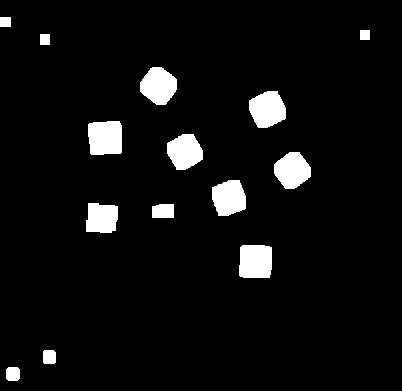
\includegraphics[width=.4\textwidth]{final_mask2.png}            
    }                                                                             
\end{figure}


\begin{figure}[H]
    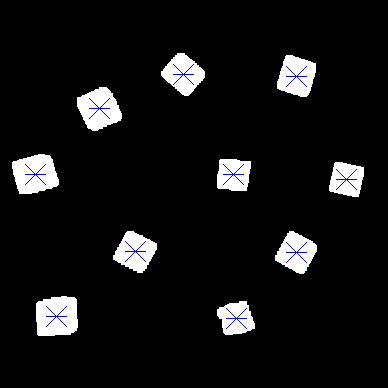
\includegraphics[width=0.4\textwidth]{figures/centroids.png}
    \caption{}
    \label{fig:centroids}
\end{figure}

\begin{figure}[H]
    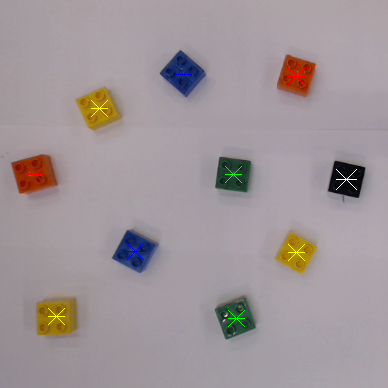
\includegraphics[width=0.4\textwidth]{figures/centroids_colour.png}
    \caption{}
    \label{fig:centroids_colour}
\end{figure}


